\newcommand{\Ca}{(0,0) ++(135:2)}
\newcommand{\Cb}{(0,0) ++(45:2)}
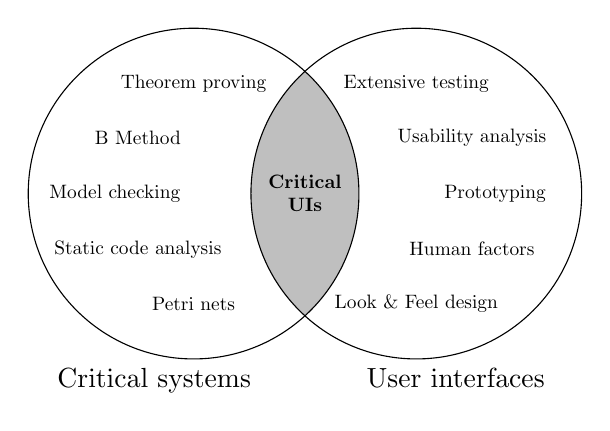
\begin{tikzpicture}
\begin{scope}
\clip \Cb circle (2.1);
\fill[lightgray] \Ca circle (2.1);
\end{scope}
\draw \Ca circle (2.1); % A
\draw \Ca ++(-0.5,-2.1) node [below] {Critical systems} ;
\draw \Ca ++(180:1) node [scale=0.7] {Model checking} ;
\draw \Ca ++(135:1) node [scale=0.7] {B Method} ;
\draw \Ca ++(-135:1) node [scale=0.7] {Static code analysis} ;
\draw \Ca ++(90:1.4) node [scale=0.7] {Theorem proving} ;
\draw \Ca ++(-90:1.4) node [scale=0.7] {Petri nets} ;
\draw \Cb circle (2.1); % B
\draw \Cb ++(0.5,-2.1) node [below] {User interfaces} ;
\draw \Cb ++(0:1) node [scale=0.7] {Prototyping} ;
\draw \Cb ++(45:1) node [scale=0.7] {Usability analysis} ;
\draw \Cb ++(-45:1) node [scale=0.7] {Human factors} ;
\draw \Cb ++(90:1.4) node [scale=0.7] {Extensive testing} ;
\draw \Cb ++(-90:1.4) node [scale=0.7] {Look \& Feel design} ;
\draw (0,0) ++(45:1) ++(135:1) node [text centered, rotate=0, scale=0.7, text width=1.7cm] {\bf Critical UIs} ;
\end{tikzpicture}
